\DocumentMetadata{pdfstandard=A-2b} 
\documentclass[11pt,a4paper]{article}
%\usepackage{swungdash}
\usepackage[top=36mm,bottom=66mm,left=40mm,right=40mm]{geometry}
\usepackage[british]{babel}
\usepackage[british]{datetime2}
\newcommand{\RNum}[1]{\uppercase\expandafter{\romannumeral #1\relax}}
\setlength{\parindent}{1em}
\DTMlangsetup[en-GB]{ord=omit}
\input{/Users/ezgranet/Desktop/stationery/ezgranet-fonts/ezgranet-fonts.tex}\directlua{}
\usepackage{titlesec}
\titleformat{\subsection}{\normalfont\centering\itshape}{\makebox[1cm][l]{\thesubsection}}{0pt}{}
\usepackage{setspace}
\newfontface\klmsctt{Morris Roman}
\usepackage[usestackEOL]{stackengine}
\usepackage[percent]{overpic}
\renewcommand{\thesubsection}{§ \arabic{subsection}}
\makeatletter
\renewcommand\tableofcontents{%
  \null\hfill\textit{\contentsname}\hfill\null\par
  \@starttoc{toc}%
}

\makeatother
\makeatletter
\renewcommand\@dotsep{200}
\makeatother

\newcommand{\catchorn}{{\addfontfeature{Ornament=44}•}}
%%%%%%%%%%%%%%%%%%%%%%%%%%%
%%%%%%%%%%%%%%%%%%%%%%%%%%%
% setup
%%%%%%%%%%%%%%%%%%%%%%%%%%%
%%%%%%%%%%%%%%%%%%%%%%%%%%%
\usepackage{hyperref}
\hypersetup{
hidelinks,
pdftitle={$title$},
pdfsubject={$description$},
pdfauthor={$author$},
pdfkeywords={$for(tags)$ $tags$ , $endfor$
}
}
\usepackage{pdfcomment}
\usepackage{pdfpages}

\usepackage{coolfn}
\usepackage{lettrine}
\setcounter{DefaultLines}{2}
\renewcommand{\DefaultLraise}{0.1}
\newcommand{\intl}[2]{\lettrine{\wtrsalt#1}{\hspace{1ex}#2}}

\usepackage{graphicx}
\usepackage{xcolor}
\definecolor{crmsn}{rgb}{0.75, 0.0, 0.2}
\definecolor{lightgrey}{rgb}{0.44, 0.5, 0.56}
\usepackage{textcsc}
\renewcommand{\textcsc}[1]{\textsc{\cscshape #1}}

\usepackage{fancyhdr,lastpage}
\renewcommand{\headrulewidth}{1pt}
\renewcommand{\footrulewidth}{1pt}
\renewcommand{\headrule}{\hrule width \textwidth height \headrulewidth \vskip 1.25pt \hrule width \textwidth height \headrulewidth \vskip -.75pt}
\renewcommand{\footrule}{\hrule width \textwidth height \footrulewidth \vskip 1.25pt \hrule width \textwidth height \footrulewidth \vskip -6pt}
\newcommand{\theotherheadrule}{{\hrule width \textwidth height \headrulewidth \vskip 1.25pt \hrule width \textwidth height \headrulewidth} \vskip 1pt}
\newcommand{\theotherfootrule}{\vskip 4pt  {\hrule width \textwidth height \footrulewidth \vskip 1.25pt \hrule width \textwidth height \footrulewidth}}

\futurelet\TMPheadrule\def\headrule{{\TMPheadrule}}
\futurelet\TMPfootrule\def\footrule{{\TMPfootrule}}

\fancyhead[L]{
\theotherheadrule\textcolor{white}{}}
\fancyhead[C]{\vskip 1pt{\sctitling \textcsc{Notes on the Style of the Law}}}
\fancyhead[R]{\vskip 1pt\textcolor{white}{}}
\fancyfoot[L]{\vskip -2pt 
{\phantom{.}$date$\theotherfootrule
}}
\fancyfoot[c]{\vskip -2pt{\textit{$title$
}  
}}

\fancyfoot[R]{\vskip -2pt {\thepage{} \textit{of} \pageref{LastPage}\phantom{.}
}}
\pagestyle{fancy}
\fancypagestyle{firstpage}{
\renewcommand{\headrulewidth}{0pt}
\renewcommand{\footrulewidth}{1pt}

\fancyhead[L]{} 

\fancyhead[c]{}

\fancyhead[R]{}

\fancyfoot[L]{\vskip -2pt 
{\phantom{.}}{}
}
\fancyfoot[c]{\vskip -2pt\phantom{ 
}}

\fancyfoot[R]{\vskip -2pt {\thepage{} \textit{of} \pageref{LastPage}\phantom{.}\theotherfootrule
}}
}
\usepackage{enumitem}
\setlist[description]{leftmargin=.5cm,labelindent=0cm}

%\date{\today}
\pagestyle{fancy}
\usepackage[noorphans,vskip=0.5ex]{quoting}
%\renewcommand{\quote}{\list{} d{\rightmargin=\leftmargin\topsep=0pt}\item\relax}

\begin{document}\thispagestyle{firstpage}
\begin{center}
\href{https://www.legalstyle.co.uk/}{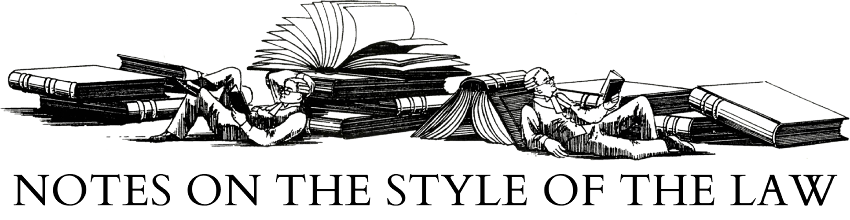
\includegraphics[width=.9\textwidth]{img/reading-bar-svg.png}}


\href{https://www.legalstyle.co.uk/}{\LARGE\textit{$title$
}}

\vskip 5pt

\normalsize\textit{by}


\href{mailto:editor@legalstyle.co.uk}{\textcsc{Elijah Z Granet}}



\vskip 6pt


{$date$}


\noindent\begin{minipage}[t]{.5\textwidth}\centering
\footnotesize%
\catchorn\ 
$for(tags)$ \href{https://www.legalstyle.co.uk/search/label/$tags$}{\textit{$tags$}} \catchorn\ $endfor$
\end{minipage}
\end{center}

\begin{center}
	
\includegraphics[width=1in]{img/fin.png}
	\end{center}
	
	
\input{$texfile$}

\begin{center}

\includegraphics[width=2in]{img/acorns-footer.png}
\end{center}

\clearpage

\mbox{}
\vfill
\begin{center}
\includegraphics[width=.3\textwidth]{caslon-border.png}
\end{center}
\begin{center}
\footnotesize\itshape This Note upon a\\matter of   legal style\\  is under the copyright\\ of the   author,\\ $year$.\\
It is licensed to all \\
 under the terms of\\
\normalfont\texttt{Creative Commons}\\
\texttt{CC-BY-SA 4.0}
\end{center}


%\vspace{.125in} 

\begin{center}
	
\footnotesize\textit{For more Notes on the}\\
\footnotesize\textit{ style of the law, visit}\\
\normalfont\href{https://www.legalstyle.co.uk/}{\footnotesize\texttt{legalstyle.co.uk}}
\end{center}

\begin{center}
\scriptsize \textit{Published}
%
%
\includegraphics[width=150px]{img/boudica-parliament-clean.png}
%
%\textit{City of Westminster}
\\
\textit{by}

\vspace*{12pt}



\includegraphics[width=.5in]{img/rs-Granet.png}

\footnotesize
\gplogo\MakeUppercase{Granet\\Press}\\
\normalfont\scriptsize\textcsc{LIMITED}
\end{center}
\begin{center}
\includegraphics[width=.3\textwidth]{caslon-border-flip.png}
\end{center}
\vfill
\end{document}